% !TEX encoding = UTF-8 Unicode

O analisador léxico atua como uma interface entre o reconhecedor sintático, que forma, normalmente, o núcleo do compilador, e o texto de entrada, convertendo a sequência de caracteres de que este se constitui em uma sequência de átomos.

Para a consecução de seus objetivos, o analisador léxico executa usualmente uma série de funções, todas de grande importância como infraestrutura para a operação das partes do compilador mais ligadas à tradução propriamente dita do texto-fonte. As principais funções são listadas abaixo:

\begin{itemize}

	\item Extração e Classificação de Átomos;
	\begin{itemize}
		\item Principal funcionalidade do analisador;
		\item As classes de átomos mais usuais: identificadores, palavras reservadas, números inteiros sem sinal, números reais, strings, sinais de pontuação e de operação, caracteres especiais, símbolos compostos de dois ou mais caracteres especiais e comentários.
	\end{itemize}
	
	\item Eliminação de Delimitadores e Comentários;
	
	\item Conversão numérica;
	\begin{itemize}
		\item Conversão numérica de notações diversas em uma forma interna de representação para manipulação de pelos demais módulos do compilador.
	\end{itemize}
	
	\item Tratamento de Identificadores;
	\begin{itemize}
		\item Tratamento com auxílio de uma tabela de símbolos.
	\end{itemize}
	
	\item Identificação de Palavras Reservadas;
	\begin{itemize}
		\item Verificar se cada identificador reconhecido pertence a um conjunto de identificadores especiais.
	\end{itemize}
	
	\item Recuperação de Erros;
	
	\item Listagens;
	\begin{itemize}
		\item Geração de listagens do texto-fonte.
	\end{itemize}
	
	\item Geração de Tabelas de Referências Cruzadas;
	\begin{itemize}
		\item Geração de listagem indicativa dos símbolos encontrados, com menção à localização de todas as suas ocorrências no texto do programa-fonte.
	\end{itemize}
	
	\item Definição e Expansão de Macros;
	\begin{itemize}
		\item Pode ser realizado em um pré-processamento ou no analisador léxico. No caso do analisador, deve-se haver uma comunicação entres os analisadores léxico e sintático.
	\end{itemize}
	
	\item Interação com o sistema de arquivos;
	
	\item Compilação Condicional;
	
	\item Controles de Listagens.
	\begin{itemize}
		\item São os comandos que permitem ao programador que ligue e desligue opções de listagem, de coleta de símbolos em tabelas de referência cruzadas, de geração, e impressão de tais tabelas, de impressão de tabelas de símbolos do programa compilador, de tabulação e formatação das saídas impressas do programa-fonte.
	\end{itemize}

\end{itemize}

Nas próximas seções definiremos com detalhes cada um dos passos para a criação e teste do analisador léxico.


\section{Descrição do funcionamento}

O analisador léxico lê um arquivo de configuração da máquina de estados
(transdutor). O mesmo pode ser comparado à seguinte regex:

\verb!(.)([^\1]*)\1\s*([A-Za-z]+(:?_[0-9]+)?)\s*([A-Za-z]+(:?_[0-9]+)?)!

Cada linha possui uma lista de caracteres delimitados por um caractere
especial (por exemplo `+' ou `\verb!#!') e dois identificadores que designam os
estados inicial e final da transição. O caractere \verb!@! designa todas as
transições, este é usado principalmente para encaminhar qualquer aceitação
final de um sub-autômato ao estado \verb!Q0!, para então ser tratado
normalmente.

Ex:
\begin{lstlisting}
+abcdefghijklmnopqrstuvxywz+    Q0      IDENT
+ABCDEFGHIJKLMNOPQRSTUVXYWZ+    Q0      IDENT
+_+                             Q0      IDENT
\end{lstlisting}
Este exemplo vai reconhecer todos os caracteres a-z e A-Z mais o underscore
(\_) como transições do estado \verb!Q0! e \verb!IDENT!.

Após a leitura do arquivo de configuração e de um arquivo com
    \emph{keywords}, faz-se a leitura do arquivo fonte, por meio do
transdutor, percorrendo-se o arquivo fonte token a token. Uma função
\verb!next_useful_token! oferece o não retorno dos tokens de espaço, tal qual a
quebra de linha e espaços normais, além de ignorar comentários. O motor do lex também substitui classes
\verb!IDENT! para \verb!RESERVED! se a palavra se encontra na lista de
identificadores reservados. 

\section{Autômatos finitos por \emph{Token}}

\begin{itemize}

\item DELIM: \verb!/[{}()\[\];]/!

\begin{figure}[H]
	\centering
	\begin{tikzpicture}[shorten >=1pt,node distance=5cm,on grid,auto] 
	   \node[state,initial] (q0)   {$q_0$}; 
	   \node[state,accepting](q1) [right=of q0] {$q_1$};
	    \path[->] 
	    (q0) edge[bend left=80]   node {\{} (q1)
	    (q0) edge[bend left=50]   node {\}} (q1)
	    (q0) edge[bend right=50]  node {(} (q1)
	    (q0) edge[bend right=80]  node {)} (q1)
	    (q0) edge[bend left=25]   node {;} (q1)
	    (q0) edge[bend right=25]  node {[} (q1)
	    (q0) edge                 node {]} (q1);
	\end{tikzpicture}
	\caption{Autômato finito DELIM}
\end{figure}

\item SPACE: \verb!/[ \t\r\n\v\f]+/!

\begin{figure}[H]
	\centering
	\begin{tikzpicture}[shorten >=1pt,node distance=5cm,on grid,auto] 
	   \node[state,initial] (q0)   {$q_0$}; 
	   \node[state,accepting](q1) [right=of q0] {$q_1$};
	    \path[->] 
	    (q0) edge   node {
			[ $\backslash$t$\backslash$r$\backslash$n$\backslash$v$\backslash$f]
		} (q1)
		(q1) edge[loop above]  node {
			[ $\backslash$t$\backslash$r$\backslash$n$\backslash$v$\backslash$f]
		} (q1);
	\end{tikzpicture}
	\caption{Autômato finito SPACE}
\end{figure}

\item COMMENT: \verb!/#[^\n]*/!

\begin{figure}[H]
	\centering
	\begin{tikzpicture}[shorten >=1pt,node distance=3cm,on grid,auto] 
	   \node[state,initial] (q0)   {$q_0$}; 
	   \node[state,accepting](q1) [right=of q0] {$q_1$};
	    \path[->] 
	    (q0) edge  node {\#} (q1)
		(q1) edge[loop above]  node {$[\hat{~}\backslash n]$} (q1);
	\end{tikzpicture}
	\caption{Autômato finito COMMENT}
\end{figure}

\item IDENT: \verb!/[a-zA-Z_][a-zA-Z0-9_]*/!

\begin{figure}[H]
	\centering
	\begin{tikzpicture}[shorten >=1pt,node distance=3cm,on grid,auto] 
	   \node[state,initial] (q0)   {$q_0$}; 
	   \node[state,accepting](q1) [right=of q0] {$q_1$};
	    \path[->] 
	    (q0) edge  node {[a-zA-Z\_]} (q1)
	    (q1) edge [loop above] node {[a-zA-Z0-9\_]} (q1);
	\end{tikzpicture}
	\caption{Autômato finito IDENT}
\end{figure}

\item INTEGER: \verb!/[0-9]+/!

\begin{figure}[H]
	\centering
	\begin{tikzpicture}[shorten >=1pt,node distance=3cm,on grid,auto] 
	   \node[state,initial] (q0)   {$q_0$}; 
	   \node[state,accepting](q1) [right=of q0] {$q_1$};
	    \path[->] 
	    (q0) edge  node {[0-9]} (q1)
	    (q1) edge [loop above] node {[0-9]} (q1);
	\end{tikzpicture}
	\caption{Autômato finito INTEGER}
\end{figure}

\item FLOAT: \verb!/[0-9]*\.[0-9]+/!

\begin{figure}[H]
	\centering
	\begin{tikzpicture}[shorten >=1pt,node distance=2cm,on grid,auto] 
	   \node[state,initial] (q0)   {$q_0$}; 
	   \node[state](q1) [right=of q0] {$q_1$};
	   \node[state,accepting](q2) [right=of q1] {$q_2$};
	    \path[->] 
	    (q0) edge  node {.} (q1)
	    (q1) edge  node {[0-9]} (q2)
	    (q0) edge [loop above] node {[0-9]} (q0)
	    (q2) edge [loop above] node {[0-9]} (q2);
	\end{tikzpicture}
	\caption{Autômato finito FLOAT}
\end{figure}

\item CHAR: \verb!/'(?:\\[0abtnvfre\\'"]|[\x20-\x5B\x5D-\x7E])'/!

\begin{figure}[H]
	\centering
	\begin{tikzpicture}[shorten >=1pt,node distance=2cm,on grid,auto] 
	   \node[state,initial] (q0)   {$q_0$}; 
	   \node[state] (q1) [right=of q0] {$q_1$}; 
	   \node[state] (q2) [right=of q1] {$q_2$}; 
	   \node[state] (q3) [right=of q2,xshift=+2cm] {$q_3$}; 
	   \node[state, accepting] (q4) [right=of q3] {$q_4$}; 
	    \path[->] 
	    (q0) edge  node {$`$} (q1)
	    (q1) edge[bend left=60] node {
	        [$\backslash$x20-$\backslash$x5B$\backslash$x5D-$\backslash$x7E]
	    } (q3)
	    (q1) edge node {$\backslash$} (q2)
	    (q2) edge node {[0abtnvfre$\backslash\backslash$"']} (q3)
	    (q3) edge node {$`$} (q4);
	\end{tikzpicture}
	\caption{Autômato finito CHAR}
\end{figure}

\item STRING: \verb!/"(?:\\"|[^"])*"/!

\begin{figure}[H]
	\centering
	\begin{tikzpicture}[shorten >=1pt,node distance=2cm,on grid,auto] 
	   \node[state,initial] (q0)   {$q_0$}; 
	   \node[state] (q1) [right=of q0] {$q_1$}; 
	   \node[state, accepting] (q2) [right=of q1] {$q_2$}; 
	    \path[->] 
	    (q0) edge  node {$"$} (q1)
	    (q1) edge [loop above] node {$[\hat{~}"]$} (q1)
	         edge [loop below] node {$\backslash"$} (q1)

	    (q1) edge  node {$"$} (q2);
	\end{tikzpicture}
	\caption{Autômato finito STRING}
\end{figure}

\item OPER: \verb$/[\+\-\*\/%=!<>][=]?/$

\begin{figure}[H]
	\centering
	\begin{tikzpicture}[shorten >=1pt,node distance=7cm,on grid,auto] 
		\centering
	    \node[state,initial] (q0)   {$q_0$}; 
	    \node[state,accepting](q1) [right=of q0] {$q_1$};
	    \node[state,accepting](q2) [right=of q2] {$q_2$};
	    \path[->] 
	    (q0) edge   node {$+$} (q1)
	    (q0) edge[bend right=65]  node {$-$} (q1)
	    (q0) edge[bend left=65]   node {$*$} (q1)
	    (q0) edge[bend right=45]  node {$/$} (q1)
	    (q0) edge[bend left=45]   node {$\%$} (q1)
	    (q0) edge[bend right=30]  node {$!$} (q1)
	    (q0) edge[bend left=30]   node {$<$} (q1)
	    (q0) edge[bend left=15]   node {$>$} (q1)
	    (q0) edge[bend right=15]  node {$=$} (q1)
	    (q1) edge   node {$=$} (q2);
	\end{tikzpicture}
	\caption{Autômato finito OPER}
\end{figure}

\end{itemize}

\section{Autômato finito único}

\begin{itemize}
    \item C\_DELIM $= [91, 93, 123, 125, 40, 41, 59]$
    \item C\_SPACE $= [32, 9, 10, 11, 12, 13]$
    \item C\_OPER  $= [42, 37, 60, 62, 43, 61, 33, 47, 45]$
    \item C\_LETTERS  $= [65, \dots, 90, 97, \dots, 122, 95]$
    \item C\_NUMBERS  $= [48, 57]$ 
\end{itemize}
\resizebox{400px}{400px}{
    \centering
\begin{tikzpicture}[shorten >=1pt,node distance=5cm,on grid,auto] 


    \node[state,initial] (q0)   {$q_0$}; 
    \node[state,accepting](delim) [right=of q0, yshift=130, xshift=-100] {delim};
    \node[state](comm) [right=of q0, yshift=100, xshift=-210] {comm};
    \node[state,accepting](comm2) [above=of comm, yshift=-30] {$comm_2$};
    \node[state,accepting](space) [right=of q0, yshift=100, xshift=20] {space};
    \node[state,accepting](oper) [right=of q0, yshift=20, xshift=40] {oper};
    \node[state,accepting](oper2) [right=of oper] {$oper_2$};
    \node[state,accepting](ident) [right=of q0, yshift=-30, xshift=40] {$ident$};
    \node[state,accepting](ident2) [right=of ident] {$ident_2$};
    \node[state,accepting](integ) [right=of q0, yshift=-100, xshift=-100] {$int$};
    \node[state](float) [right=of integ, xshift=20] {$float$};
    \node[state,accepting](float2) [right=of float] {$float_2$};
    \node[state] (char1) [left=of q0, yshift=-60] {$char$}; 
    \node[state] (char2) [below=of char1] {$char_2$}; 
    \node[state] (char3) [below=of char2] {$char_3$}; 
    \node[state, accepting] (char4) [right=of char3] {$char_4$}; 
    \node[state] (str1) [left=of q0, yshift=60] {$str_1$}; 
    \node[state, accepting] (str2) [above=of str1] {$str_2$};
    \path[->] 

    (q0) edge node {$\#$} (comm)
    (comm) edge [loop left] node {$[\hat{~}\backslash{}n]$} (comm)
    (comm) edge node {$\backslash{}n$} (comm2)
    (q0) edge node {C\_DELIM} (delim)
    (q0) edge node {C\_SPACE} (space)
    (q0) edge node {C\_OPER} (oper)
    (oper) edge node {$=$} (oper2)
    (q0) edge node {C\_LETTERS} (ident)
    (ident) edge [bend left=19] node {C\_LETTERS $|$ C\_NUMBERS} (ident2)
    (q0) edge [bend right=19] node {C\_NUMBERS} (integ)
    (integ) edge [loop below] node {C\_NUMBERS} (integ)
    (q0) edge  [bend left=19] node {$.$} (float)
    (integ) edge node {$.$} (float)
    (float) edge  node {C\_NUMBERS} (float2)
    (float2) edge [loop below] node {C\_NUMBERS} (float2)
    (q0) edge  node {$'$} (char1)
    (char1) edge[bend left=60] node { %
        [$\backslash$x20-$\backslash$x5B$\backslash$x5D-$\backslash$x7E] %
    } (char3) 
    (char1) edge node {$\backslash$} (char2)
    (char2) edge node {[abtnvfre$\backslash\backslash$]} (char3)
    (char3) edge  node {$'$} (char4)
    (q0) edge  node {$"$} (str1)
    (str1) edge [loop left] node {$[\hat{~}"]$} (str1)
           edge [loop right] node {$\backslash"$} (str1)
           edge  node {$"$} (str2);
\end{tikzpicture}
}

\section{Trandutor léxico}

O transdutor obtido a partir do autômato finito únco pode ser visto na Figura~\ref{fig:transdutor}.

\begin{figure}
	\centering 
	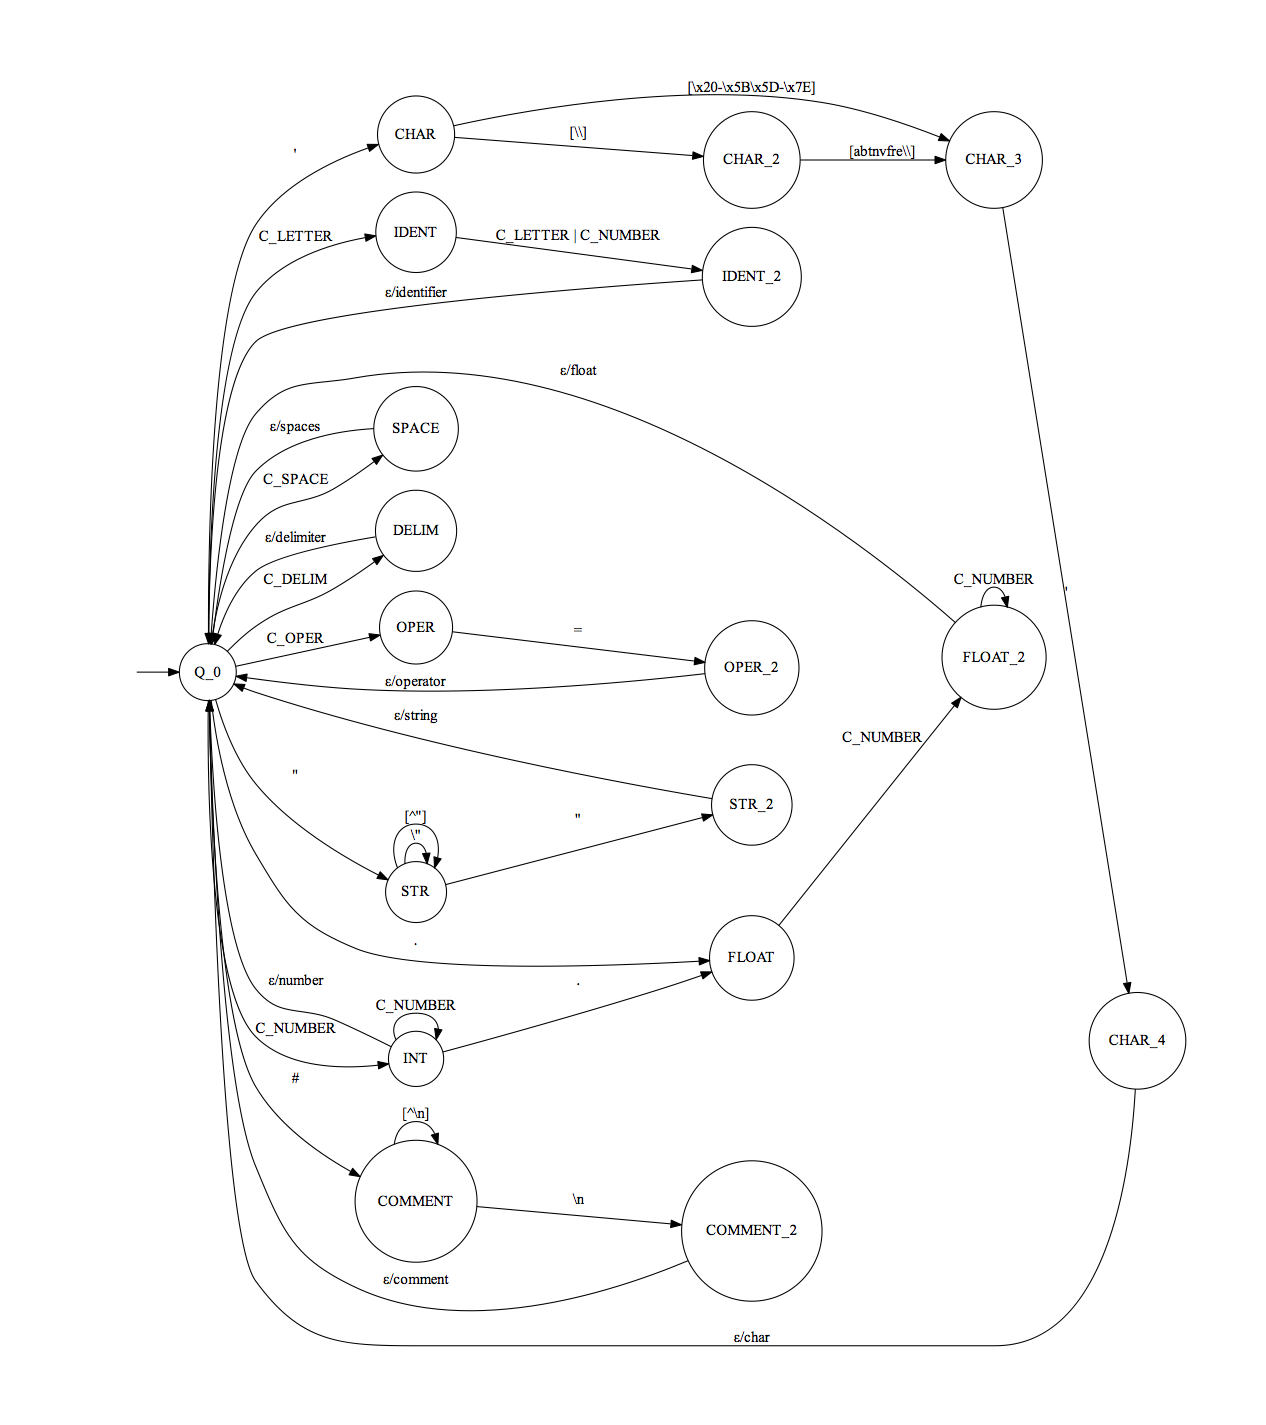
\includegraphics[width=\textwidth]{images/transdutor.png} 
	\caption{Transdutor léxico da Linguagem \emph{CZAR}}
	\label{fig:transdutor}
\end{figure}

\section{Testes}


Um código de exemplo que foi utilizado para teste está listado abaixo:

\textbf{\emph{ENTRADA.txt}}
\lstinputlisting[frame=single,language=C,numbers=left,breaklines=true]{testes_lexico/ENTRADA.txt}

Ao utilizar o código acima como \emph{input}, obtivemos o seguinte resultado, que foi de acordo com o esperado:

\textbf{\emph{Resultado sem erros}}
\lstinputlisting[frame=single,numbers=left,breaklines=true]{testes_lexico/Resultado_sem_erros.txt}

Ao introduzir um erro colocando mais de uma letra como caracter, obtivemos, como esperado, o seguinte resultado:

\textbf{\emph{Resultado com erro}}
\lstinputlisting[frame=single,numbers=left,breaklines=true]{testes_lexico/Resultado_com_erro.txt}